%\documentclass[12pt,handout]{beamer}
\documentclass{beamer}
\usepackage[ngerman]{babel}
\usepackage[utf8]{inputenc}
\usepackage{amsmath}
\usepackage{amssymb}
\usepackage{listings} 
\usepackage{stmaryrd}
\lstset{language=Python, tabsize=4, showstringspaces=false,basicstyle=\tiny,mathescape=true}
\lstset{literate=%
  {Ö}{{\"O}}1
  {Ä}{{\"A}}1
  {Ü}{{\"U}}1
  {ß}{{\ss}}1
  {ü}{{\"u}}1
  {ä}{{\"a}}1
  {ö}{{\"o}}1
}
\usepackage{mathtools}
\usepackage{ulem}
\usepackage{tikz}

\usetheme{Boadilla}
\mode<presentation>{
\useoutertheme[subsection=false]{miniframes}
\useinnertheme{rectangles}
%\usecolortheme{crane}
}
\parskip 10pt

\begin{document}
\title{Informatik}   
\author{Hashing} 
\date{}
\frame{\titlepage} 

%---
\begin{frame}[fragile]


Zum Abspeichern und Wiederfinden von Objekten wäre folgende Funktion hilfreich: 

 f: Objekte $ \rightarrow \mathbb{N}$ 

Dann könnte Objekt x unter Adresse f(x) gespeichert werden. 

f heißt Hashfunktion. \pause

Problem: Anzahl Objekte ist möglicherweise größer als die Anzahl der Adressen.  

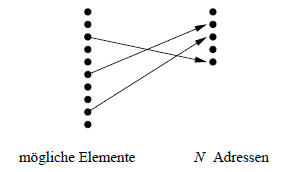
\includegraphics[scale=0.6]{bild1.png}  

Kollision: wenn $f(x) = f(y)$ für $x \ne y$ 
\end{frame}

%---
\begin{frame}[fragile]

Beispiel einer einfachen Hashfunktion. 

Gegeben seien die Adressen von 0 bis $N-1$.  

f: Menge der Strings $\rightarrow \{0,....,N-1\}$ \pause

f(s) = (Summe aller ASCII-Codes der Zeichen von s ) \% N \pause

Für beliebige Objekte x könnte f für die String-Repräsentation \texttt{x.\_\_str()\_\_} einen Wert berechnen.

Diese Hashfunktion funktioniert in vielen Fällen schon ganz gut, wenn N eine Primzahl ist, die nicht nahe bei Potenzen von 2 oder 10 liegt.

%Bessere Hashfunktion: $h(k) = ((ak+b) \%p) \% N$ \\
%p Primzahl $>$ Anzahl zu hashender Objekte,\\
%a, b zufällig gewählt aus ${0,1...,p-1}$. 
\end{frame}


%---
\begin{frame}[fragile]
Offenes Hashing \pause

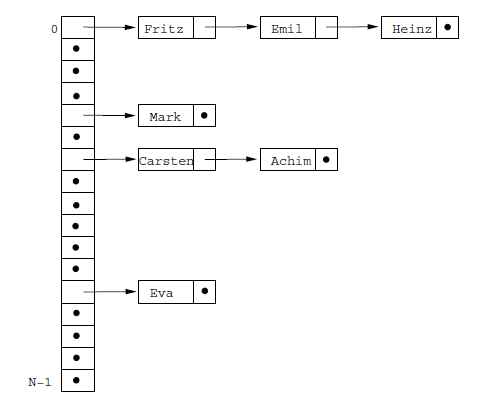
\includegraphics[height=6cm]{bild2.png}  


Datenstruktur für die Implementierung: ein Liste von Listen (ein Array von verketteten Listen)

\end{frame}


%---
\begin{frame}[fragile]
Geschlossenes Hashing \pause

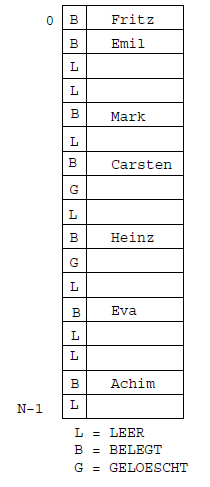
\includegraphics[scale=0.6]{bild3.png}  

Datenstruktur für die Implementierung: eine Liste für die Objekte und eine für die Zustände.
\end{frame}

%---
\begin{frame}[fragile]
Sondierung: wenn $y = f(x)$ schon belegt, so suche für x einen Alternativplatz 

\begin{itemize}
\item lineares Sonderieren: $y+1, y+2, y+3, y+4 .... $ 

\item quadratisches Sondieren: \pause $y+1, y+4, y+9, y+16 , ....$  

\item double Hashing: \pause  $y + f_2(x), y + 2 \cdot f_2(x), ... $  die Schrittweite wird durch eine 2. Hashfunktion bestimmt.\pause
\end{itemize}

Alle Berechnungen werden jeweils mod(N) durchgeführt. Beim quadratischen Sondieren werden ggf. nicht alle Buckets besucht.  

Eine \textit{perfekte} Hashfunktion verursacht keine Kollisionen.

\end{frame}

%---
\begin{frame}[fragile]
Laufzeit bei geschlossenem Hashing  

N = Anzahl der möglichen Speicherpositionen, n = Anzahl der gespeicherten Objekte

$\alpha = \frac{n}{N}$ heißt Belegungsgrad oder Auslastungsfaktor. 

Als durchschnittliche Anzahl der Sondierungsschritte bei Double-Hashing ergibt sich bei  

\begin{itemize}
\item erfolgloser Suche: $\approx \frac{1}{1-\alpha} = 5$  für $\alpha = 0.8$  
\item erfolgreicher Suche: $\approx \frac{\ln(1-\alpha)}{\alpha} = 2.01$ für $\alpha = 0.8$ \pause
\end{itemize}

d.h. in 2 Schritten wird von 1.000.000 Elementen aus einer 1.250.000 großen Tabelle das richtige gefunden. Ein ausgeglichener Suchbaum benötigt dafür etwa 20 Vergleiche. 
\end{frame}

%---
\begin{frame}[fragile]
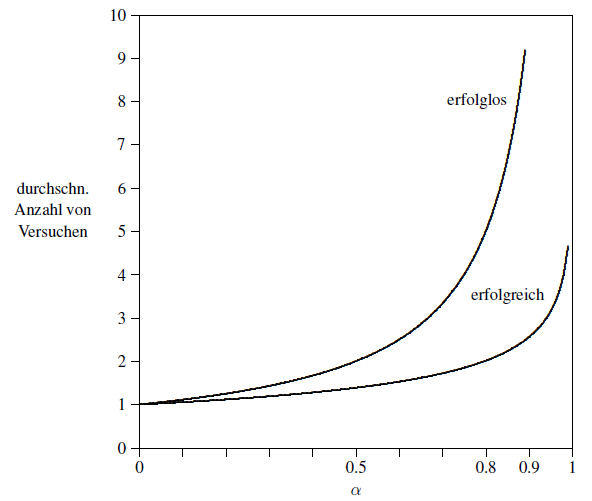
\includegraphics[scale=0.5]{bild4.png}  

\begin{tabular}{lll}
& ausgeglichener Suchbaum & geschlossenes Hashing  \\ 
\hline
Laufzeit  & logarithmisch & konstant \\ 
Speicherbedarf  & dynamisch wachsend & in Sprüngen wachsend \\
Sortierung & durch Traversierung &- \\
\hline
\end{tabular}
\end{frame}
 \end{document}